\chapter{Introduction}

\section{Motivation}

\section{Idea}

\section{Contribution}

\section{Outline}

\chapter{Background}

In this chapter we will cover concepts relevant for the rest of the paper. %TODO continue

\section{Malware}

The word \emph{malware} is a blend word for malicious software. As such, it is an umbrella term which encompasses any type of software which is intentionally designed to disturb the intended use, or operation of a computer system, without the explicit permission of its user(s) or owners. The goal of a piece of malware can include, but is not limited to: leakage or collection of private information, restriction of access to data with the goal of monetary gains, network overload, device hijacking, espionage, serving of targeted adds \cite{wiki_malware}.

\subsection{Classification}

Malware are typically grouped by their behaviour and/or purpose and could fall under one or more of the labels in the following non-exhaustive list: backdoor, bot(net), dropper, fileless, ransomware, rootkit, spyware, trojan, virus, worm, etc. We will shortly cover the most relevant ones as follows \cite{wiki_malware}, \cite{zeusvm}.

\subsubsection{Backdoor}

A Backdoor is an umbrella term depicting programs that enable bad actors to obtain persistent, unauthorised access on a victim's computer, typically without them being aware of the situation. Backdoor are interesting, because they can either be delivered through a Trojan, a worm, or another similarly purposed malware, but they can also be the result of vulnerabilities existing in legitimate software, that already exist on the victim's computer. What is more, there also a combined scenario, where a backdoor is intentionally inserted into legitimate software. This can be done, for instance, by a bad actor hiding their intension. This was the case, for instance, with the 2024 discovery of the XZ Utils backdoor \cite{xz_backdoor}.

\subsubsection{Trojan}

A Trojan, or a Trojan Horse, is a type of malware that concals itself inside another program that appears benign. It typically misinforms the target about its behaviour in order to persuade a victim to install it on their computer. Trojans are usually delivered by some form of social engineering. The payload of a Trojan can be anything. It often is another type of malware, case in which, the Trojan is considered a Dropper. It can also be the case that the Trojan deploys a backdoor which can enable unauthorised control of the infected system to a third party actor.

\subsubsection{Worm / Virus}

Worms and viruses are simmilar in the sense that these are both standalone malware that have the capacity to spread through a network, and to infect other victims. A virus (inspired from the biologial term) will inject itself simmingly harmless programs, which upon execution will further spread the infection. Worms differ from viruses in the sense that a virus requires the victim to execute the infected software in order for it to spread, whereas a worm does not. Worms can spread without user intervention and without modifying other files on the system \cite{wiki_malware}. An example of such a piece of malware is the infamous Stuxnet virus \cite{stuxnet}.

\subsubsection{Ransomware}

Ransomware is a type of malware that, once it infected a computer, restricts access to information on that particulat machine, and then requires a ransom from the victim, in exchange from the locked up information. Most comonly, a form of encryption is applied to the restricted data, which in properly executed attacks cannot be recovered without the encryption key. Typically, ransomware is delivered via a Trojan, but this is not always the case. The infamous \emph{WannaCry} ransomware was a \emph{worm} which spread through the network without user intervention \cite{wiki_wannacry}, \cite{wiki_ransomware}. As it can be seen in Figure \ref{fig:wannacry}, the attackers will ask for hard to trace digital currencies, such as Bitcoin in this case.

\begin{figure}[h]
    \centering
    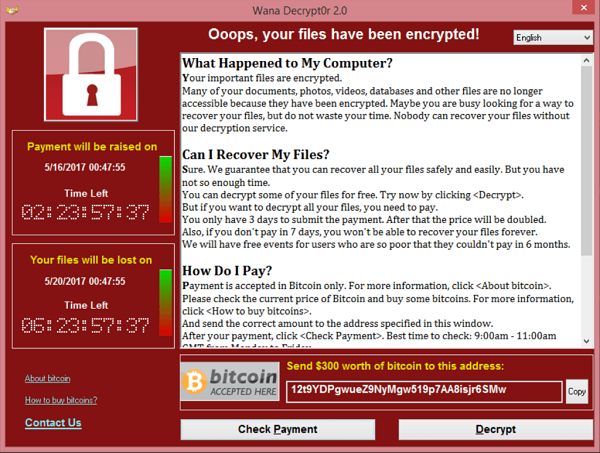
\includegraphics[width=0.8\textwidth]{./images/wanacry.png}
    \caption{An infamous screenshot of the ransom pop-up which would show up on a system infected by the WannaCry worm \cite{wiki_wannacry}.}
    \label{fig:wannacry}
\end{figure}

\subsubsection{Bot and Botnets}

A bot is a computer infected by a specific type of malware which enables its victim to be remotely controlled. Such malware is spread with the goal of infecting as many targets as possible. The infected machines are added to a common pool, called a \emph{botnet}, which can be orchestrated from a \gls{CC} center to perform other malicious activities on a bigger scale. The Andromeda botnet is an example of such malware \cite{andromeda} \cite{kaspersky_malware_types}.

\subsection{Relevance}

Malware attacks, which we will further refer to with the broader term of cybercrime, can target governments, corporations, public figures, or individuals. Multiple sources, including a report from the World Economic Forum \cite{wef_cybercrime}, suggest that cybercrime continues to rise both in numbers as well as in damage. The estimated costs of cybercrime in 2023, at a global scale, are of \$11.5 trillion, and these numbers are expected to more than double in the next 5 years. Because of this, malware, and particularly the subject of malware analysis, are evermore relevant.

\section{Reverse Engineering} % TODO obv change this
\label{sec:reverse_engineering}

% TODO: this passage is nice : > Also, a discipline that may be used to any area of forward engineering; it is analogous to scientific research except that the study is performed on a man-made product rather than a natural event.

As stated on \emph{Wikipedia}: \emph{``Reverse engineering is a process or method through which one attempts to understand through deductive reasoning how a previously made device, process, system, or piece of software accomplishes a task with very little (if any) insight into exactly how it does so''} \cite{re_wiki}.

In this work we will focus on reverse engineering pieces of software in the context of performing security research or malware analysis. Typically, in such contexts, the goal is to understand the behaviour of a piece of software, without having access to its source code. Depending on the type of analysis, a reverse engineer might have different approaches. 

They might focus on gaining a comprehensive understanding of specific parts of the software in order to identify weaknesses, or more commonly named \emph{vulnerabilities}. The analysis could be restricted to specific parts because for multiple reasons which include, but are not limited to: the full program being to big to justify performing a full analysis, or the existence of prior knowledge which gives higher priority to the analysis of certain code regions. With the knowledge obtained from RE, the engineer can identify and prove the existence of attack vectors on a system that is running this software. They might then write a report which covers the risks to which entities running the software are exposed, describing in detail the finding and, eventually exemplifying how an attacker might abuse the discovered vulnerabilities. In this case, the end goal is to initiate the process of patching the vulnerable piece of software. % TODO might want to cite here

In other instances, the engineers might perform a full and comprehensive analysis of piece of software. This is typically done when dealing with malware. The malware analyst will first try to determine if the piece of software is in fact malicious or not. If the code is malicious, it is important to determine its behaviour, how it interacts with the system, or with outside entities (possibly by creating network traffic). Further, analysts might study and document novel techniques employed by attackers. They might also integrate the newly find malware into a detection system to prevent future uses of the respective malware \cite{malware_crowdstrike}.

Regardless of the goal, RE falls into one of two broad categories which determine the typical approach and the tooling used: \textbf{static analysis} and \textbf{dynamic analysis}.

\section{Static Analysis}

Static analysis represents the multitude of techniques employed to analyse a program without executing it. These techniques range in difficulty and complexity starting from reading source code, to reading assembly, attempting to decompile the binary and ultimately to using very advanced tools and theoretical knowledge such as \gls{SE} engines, SMT solvers or formal methods. %TODO I am not sure anylonger if SE should be included here or not

In its most basic form, static analysis is equivalent with reading the source code in order to understand what the program does. However, in the context of this paper, we are dealing with binary files, compiled to machine code. The source code is not available to us, so we must resort to other analysis techniques. One option is to convert the machine code into the human readable form, called assembly. The process is known as machine code disassembly. Assembly code is typically very hard to understand for humans, but from it the logic of the program can be successfully recovered, given enough time and effort. One advantage of static analysis through reading assembly is that the entry barrier is not high in terms of the tooling required. A very basic tool such as \cc{objdump} \cite{TODO} can be enough for simple programs, but most likely a more feature rich tool such as \cc{radare2}/\cc{cutter} \cite{TODO} might be more suitable, as these are able to display basic blocks and how all such \gls{BB} relate to each other and form the \glspl{CFG}.

Reverse engineers typically default to more advanced static analysis tools, such as IDA or Ghidra. These tools feature a suite of functionalities, out of which, probably the most prominent is the \emph{decompiler}. Compilation is the process of converting source code into machine code. Decompilation is the opposite: the process of converting machine code, back into source code. Compared to the disassembly process, which is deterministic and corresponds exactly to the assembly process, the decompilation process will almost never yield back the original source code. This is the case because a lot of information useful to programmers, but useless for the \gls{CPU} is lost during the compilation process. This information includes, but is not limited to: variable and function names, type information, custom defined data types such as structures, or specific language features. This is why decompilers will always output an approximation of the original code. 

Let us consider a concrete example and consider Listings \ref{code:decompilation-original}, \ref{code:decompilation-1}, \ref{code:decompilation-2}. Listing \ref{code:decompilation-original} contains the implementation of the function \cc{add}, which takes the end of linked list and a value, and creates a new node in the list with that value, also taking the necessary steps to update the list accordingly. The code is part of a slightly larger \cc{C} program, which we compiled and imported into Ghidra. Looking at Listing \ref{code:decompilation-1} we can see the decompilation of the exact code in the previously mentioned listing. It is immediately obvious that: the type information related to \cc{node} structure is completely lost and that the original function was inlined by the compiler. As a result, the decompilation is an obfuscated version of the original code. This is a well known fact and advanced tools such as Ghidra offer various features, which the reverse engineer can utilise in order to remove part of the obfuscation. Listing \ref{code:decompilation-2} contains the same segment of decompiled code after a minimal amount of manual intervention, which includes: variable renaming, custom type creation and type updates. Clearly, it is a lot more human readable and bears a closer resemblance to the original code in Listing \ref{code:decompilation-original}. 

Decompilers and disassemblers are very powerful tools, which aid significantly in the process of static analysis. However, these tools have their shortcomings as highlighted above. Moreover, there are certain program behaviours which cannot, or are significantly harder to understand only by \emph{looking} at the code.

% Found a paper which I can use to add more about this :D
% see static analysis techniques 2015

% TODO mention techniques which hinder static analysis

\begin{lstlisting}[language=c, label={code:decompilation-original}, caption={A function which adds an integer value \cc{v} to the end of a linked list.}]
void add(lnode** node, int v) {
    // allocate memory for a new node in the liked list
    lnode* new_node = (lnode*) malloc(sizeof(lnode));
    new_node->val = v; // set the value
    if (*node != NULL) {
        (*node)->nxt = new_node; // link to the new node from the end of the list
        *node = new_node; // move the list end to the new node
    } else {
        *node = new_node; // TODO fix comments set it as the end of the list, it it is the first one
    }
}
\end{lstlisting}

\begin{center}

\begin{minipage}[5]{0.45\textwidth}
\begin{lstlisting}[language=c, label={code:decompilation-1}, caption={Ghidra decompilation of the code presented in Listing \ref{code:decompilation-original}. The decompilation is take as-is and has not modified in any way.}]
piVar1 = (int *)malloc(0x10);
*piVar1 = iVar3;
if (piVar5 != (int *)0x0) {
    *(int **)(piVar5 + 2) = piVar1;
}
piVar5 = piVar1;
if (piVar4 == (int *)0x0) {
    piVar4 = piVar1;
}
\end{lstlisting}
\end{minipage}
\hspace{1.3cm}
\begin{minipage}[5]{0.45\textwidth}
\begin{lstlisting}[language=c, label={code:decompilation-2}, caption={Ghidra decompilation of the code presented in Listing \ref{code:decompilation-original}. The decompilation has been modified by renaming variabled and changing data types, based on educated guesses.}]
new_node = (node *)malloc(0x10);
new_node->val = v;
if (last_node != (node *)0x0) {
    last_node->nxt = new_node;
}
last_node = new_node;
if (root == (node *)0x0) {
    root = new_node;
}
\end{lstlisting}
\end{minipage}

\end{center}

\section{Dynamic Analysis}

As described by T. Ball in his 1999 paper \cite{concept_of_da_1999}, \emph{``dynamic analysis is the analysis of a running program''}. This type of analysis is desirable in different situations where static analysis could not extract sufficient information, or when acquiring extra information depends the program to be running %TODO i could give more examples here, relating to why static analysis cannot work in certain situations. also should mention for the static analysis part exactly this. probably will need to talk before RE about obfuscation techniques. OR NOO!! I can talk right after, in order to present some means to prevent static analysis
Dynamic analysis is an umbrella term which covers many powerful techniques used for program analysis. A taxonomy of these techniques has been presented in a comprehensive survey by Ori et al. in 2019 \cite{da_survey_2019}. We will shortly cover some of them.

\subsection{Debugging}

% TODO define somewhere that we'll be referring to a reverse engineer / malware analysit as "the analyst" throughout this work

Debugging is a very well known technique, especially popular among developers who use it mainly to identify bugs or errors in their code. It is however a very effective and reliable form of analysing unknown programs (eg. malware). Also called \emph{single stepping}, it involved using a tool, intuitively called a \emph{debugger}, in order to run the program one instruction at a time. After each instruction, the analyst can inspect the state of the registers, the memory and what instructions follow. This process can also help in determining any relevant changes in the operating system itself, caused or related to the debugged program.

Debuggers use the CPU's trap flag in order to trigger an interrupt after each instruction, or only certain desired instructions. The interrupt causes a context switch from the execution of the debugged program to the debugger. To continue execution, the trap flag is set again and the context switches back to the program. The high number of context switches means that debugging is a very resource intensive analysis technique. It is also very easy to detect by the running malware, which can check the state of the trap flag and hide its behaviour in case it is debugged \cite{da_survey_2019}.

\subsection{Function Call Analysis}

% TODO explain what a syscall is?

Any type of meaningful action that a malware can take, will ultimately rely on system calls. It can be the case that these system calls are performed through function calls from an external library, such as the standard \cc{libc} library, or from an internally defined function. Analysing function calls, the state of the program before, during and after the function call, as well as the parameters used can provide valuable information about the behaviour of the analysed program. Techniques for approaching this goal vary. For instance, we could use command line (cli TODO) programs such as \cc{strace}, or \cc{ltrace}, which track system calls and library calls respectively. We could also use more advanced techniques, such as function hooking. An analyst can extract more information from a function call by \emph{hooking} (i.e. linking) a piece of code to the targeted function. What will happen is that upon the function call, the \emph{hooked} code will run as well, which can just print debugging messaged to inform the analyst that the function has just been called, or access the state of the program at that time and save it for further inspection. \cite{da_survey_2019}

Function calls can also be used as a powerful side-channel. More specifically, one can monitor the amount of \cc{calls} which have been made since reference point in order to determine if progress has been made or not in the execution. Let's consider Listing \ref{code:ltrace}. We're running the \cc{crackme} program through \cc{ltrace} to monitor function calls, with a randomly chosen input string. We notice a length check with \cc{strlen} at Line \ref{code:ltrace-1}, after which the program crashes. By selecting the correct input length of $70$ bytes, we can pass the length check at Line \ref{code:ltrace-2}. This \cc{crackme} is a particularly good example for using this technique, because it is heavily obfuscated. We cannot effectively use static analysis on this binary, so employing dynamic analysis techniques enables us to make progress and recover the secret \cite{crusu_relabs}.

% TODO explain what a crackme is 

\begin{lstlisting}[caption={ltrace (``a library call tracer'') output of an obfuscated crackme. One can observe a length check in the first execution, and different output when an input of the expected length is provided.}, label={code:ltrace}]
>_ python -c "print('a' * 42)" | ltrace ./crackme
memset(0x8625ae8, '\0', 10000)                         = 0x8625ae8
fgets("aaaaaaaaaaaaaaaaaaaaaaaaaaaaaaaa"..., 10000, 0xf22e9700) = 0x8625ae8
strlen("aaaaaaaaaaaaaaaaaaaaaaaaaaaaaaaa"...)          = 43 @$\label{code:ltrace-1}$@
puts("WROOONG!"WROOONG!)                               = 9
exit(1 <no return ...>)
+++ exited (status 1) +++

>_ python -c "print('a' * 70)" | ltrace ./crackme
memset(0x8625ae8, '\0', 10000)                         = 0x8625ae8
fgets("aaaaaaaaaaaaaaaaaaaaaaaaaaaaaaaa"..., 10000, 0xedcf4700) = 0x8625ae8
strlen("aaaaaaaaaaaaaaaaaaaaaaaaaaaaaaaa"...)          = 71
strstr("aaaaaaaaaaaaaaaaaaaaaaaaaaaaaaaa"..., "zihldazjcn") = nil @$\label{code:ltrace-2}$@
puts("WROOONG!"WROOONG!)
exit(1 <no return ...>)
\end{lstlisting}

\subsection{Dynamic Taint analysis}

Dynamic Taint analysis is a technique used to track data flow from sources to sinks. In order to achieve this goal, data considered important is given a label (\emph{a taint}), based on a \emph{taint introduction policy}. Typically, we would taint untrusted user input or data arriving over the network. This \emph{tainted} data is propagated through the system based on execution and how the code interacts with the data at the opcode level. When an operation is performed on tainted data, memory locations used during the respective operation are also tainted, based on a \emph{taint propagation policy}. Some memory areas, or code sections are also marked as \emph{sinks}. When tainted data arrived at a sink, the path it took through the code can be traced back. In the context of malware analysis, the flow of tainted data is valuable, as it gives valuable insights about the ways the malware interacts with the user and the operating system. Taint analysis is also valuable for exploit detection, and was initially used specifically for this goal. By tainting untrusted user input one can detect unusual data flows and detect attempts at exploiting a system. In such cases, a \emph{taint checking policy} might be used to determine further behaviour (e.g. halting execution) \cite{da_survey_2019} \cite{all_about_taint_2010}.

\section{Other Approaches}

\subsection{Symbolic Execution}

% TODO asta e la static analysis teoretic

\gls{SE} is a powerful program analysis technique, and one of the core techniques which the idea of this paper is based on. As such, we will cover \gls{SE} in more detail compared to the other dynamic analysis approaches.

% TODO bat campii efectiv, trebuie sa reformulez
\gls{SE} is typically discussed in relation with \emph{\gls{CE}}. \gls{CE} is the formal term for what we refer to as normal program execution. That is, executing a program with a concrete input until the end of a single execution path. When every possible external value (user input, response from a system call, return value of a function) has a concrete value, we're dealing with \gls{CE}.
Let us consider Listing \ref{lst:fizzbuzz}. The value of the argument \cc{c} is given by the caller of the function \cc{fizzbuzz}. If we consider a concrete value of $7$ for \cc{c}, we expect the program to print the same value $7$ at the standard output, after executing Line \ref{code:fizzbuzz-1}. We can test this hypothesis by running the program, passing the respective value to the function and inspecting the printed value. This is concrete execution.

\lstinputlisting[language=c, label={lst:fizzbuzz}, caption={TODO}]{./code/fizz-buzz.tex}

In contrast with \gls{CE}, with \gls{SE} we can explore all possible paths of execution. Moreover, for each path we will have a logical condition which precisely describe the values of the inputs which will lead the execution on that specific path.

in order to determine what classes of inputs lead to which execution paths.

The key aspect of \gls{SE} is the use of symbolic values, as opposed to concrete values. Initially, the symbolic values are unconstrained, meaning that they can represent any possible input value associated to that type. The program is executed in a controlled environment by a \gls{SE} engine. The engine keeps track of a logic formula which describes the constraints that the input must satisfy, in order to follow each specific execution path that is being tracked. It also keeps trace of the symbolic memory store, which keeps track of symbolic values and memory areas, and the expressions or concrete values which these hold. As the program executes, each conditional branch splits the symbolic state into two and adds new constraints to each branch, based on the respective conditional.

\subsection{Concolic Execution} % \subsection{Mixed Approaches ???}

% TODO this paragraph does not fit here AT ALL!
% TODO find a way to repurpose it
% Typically, when running unknown software the researcher or analyst is exposing his system to the risk of being compromised. This is especially prevalent when we are dealing with potential malware. For these situations specific techniques have been devised in order to protect the host system from being infected, while still having an environment where the unknown software can be executed and its interactions with the system monitored and then analysed. Such environments are called sandboxes, and isolate the suspicious software from the main OS(TODO), in such a way that the host of the system, as well as the network are safe from infection, or compromise.

%\section{Malware Obfuscation}
\section{Obfuscation Techniques}

% TODO cite more, provide source for evading protections

Obfuscation is an umbrella term for a set of techniques, very widely employed in the field of software engineering, for protecting source code. This is done by making the code harder to understand, without changing its behaviour (semantics). Obfuscation is used, especially when the code contains \gls{PI}, which must be protected against \gls{RE}. Not surprisingly, obfuscation is very common in malware. In this case, obfuscation is used to evade automatic malware detection systems, such as anti-viruses. Moreover, many obfuscation techniques are specifically aimed at the researchers who are expected to attempt doing \gls{RE} on it, aiming to slow down the analysis, which in turn enables the bad actors to inflict more damage on their targets. \cite{zeusvm} 

\subsection{Classification}

There are a number of malware obfuscation techniques which have been observed in the wild time and time again. We will cover some of the most relevant as follows

\subsubsection{Classical Techniques}

%\subsubsection{Encryption}
%\subsubsection{Constant Unfolding}
%\subsubsection{Dead Code Insertion}
%\subsubsection{Data encoding schemes}
%\subsubsection{Pattern-based obfuscation}
%\subsubsection{Control Indirection}
%\subsubsection{Junk Code insertion}

% FIXME I hate you!!!!!

A very common way to try and evade signature-based detection is to encrypt the malicious payload. This obfuscation technique implies a couple of things. First of all there needs to exist an encryptor, which encrypts each iteration of the malware, ideally with a different key. As such the result differs between iterations. Second of all, there needs to exits a decryptor, packaged together with the malware. This is essential, because the decryptor must be triggered upon execution of the malicious code, in order for the operating system to be able to execute it. The second point constitutes a big weakness of this technique, because the antivirus could employ a strategy where it targets the signature of the decryptor.

\subsubsection{Classical Techniques}
% TODO check the book

\subsubsection{Opaque Predicates}

\subsubsection{Mixed Boolean-Arithmetic}
% TODO there is a paper somewhere about this one

\subsubsection{Control-Flow Flattening}

\subsubsection{Virtual Machines}


\cite{malware_obf}
% TODO it is important to note that techniques are not singluar and can, and often are, combined


% TODO figure out if this fits better in the next chapter (I think yes)
% TODO JUST PUT A SECTION IN THE NEXT CHAPTER
% TODO might be worth a chapter describing virtual machines and sht, but we'll see
% TODO the correct term seems to be virtualisation-based obfuscation

% TODO for getting info on VMs and other techniques: LOKI: Hardening Code Obfuscation Against Automated Attacks

\Glspl{VM} 

% ------------------------------------------------------------------------------

\chapter{State of the Art}

% TODO fix this sht here 

%There have been public a number of academic works describing various approaches to analysing protections based on virtualisation-based obfuscation. As also mentioned in one of these works by Salwan et al. \cite{symbolic_deobf_2018}, these approaches can be grouped together in categories. There are manual and (semi) manual approaches, which usually rely on an skilled reverse engineer to analyse the \gls{VM} interpretor and its bytecode. There are (semi) automatic approaches, where static and dynamic analysis techniques are applied in order to \emph{filter out} the non-essential parts of the code, and to recover the unprotected code form the result. Other approaches use Program Synthesis in order to automatically deobfuscate arithmetic and \gls{VM} handlers % TODO, in a common programming language. THIS IS KINDA SHTTT

% chronological order -> chronological classification if there is any separation - and i think there is !!

In these chapter, cover the main contributions of recent pieces of work. At the end of the chapter we will discuss how the state of the art compares with our approach.

\section{Virtualization-based Obfuscation}

\section{Semi-Manual Approaches}

One of the first academic works on the topic roots back to 2009, when Rolles \cite{rolles2009unpacking} published a systematic approach to tackling virtualisation-based obfuscation. The authors describe a multi-step strategy to recover the original source code from the protected program. They start with analysing the \gls{VM} interpretor in order to recover the semantics of the handlers. They use this information in order to construct an \gls{IR} which to lift the \gls{VM} bytecode into, as well as a translator which takes care of the translation automatically. As mentioned by the authors, this step must be executed by a professional reverse engineer, and must be performed once for each virtualisation scheme which is to be analysed. They process with identifying the exact location in the code where control is passed to the \gls{VM} interpretor. The multiple steps that follow in the process involve building the disassembler, disassembling the bytecode. On the resulting bytecode is simplified using compiler optimisation techniques, and finally the code is translated into \cc{x86} \gls{ISA}, with the end goal of recovering code as close to the original as possible. The strategy proposed in this work is very effective, but requires significant reverse engineering effort.

\section{Semi-Automated Approaches}

Sharif et al introduce in 2009 the Rotalumé framework \ref{sharif2009}, which they claim to be the first work aiming to automatically deobfuscate virtualised malware. In their prototype, they execute chosen samples using the using QEMU \cite{qemu}, in order to capture its execution trace in a protected environment. Using the execution trace, they were able to automatically detect the bytecode buffers and extract the syntax and semantics of the bytecode, by applying data-flow and taint analysis. The Rotalumé framework is able to construct the \gls{CFG} of the program encoded in the bytecode, an important element of following analysis.

In 2015, Yadegari et al. proposed a generic approach to deobfuscating programs \cite{yadegari2015}. They do not make any assumptions about the nature of the obfuscation, but claim their method is effective against a wide array of obfuscation techniques, including virtualisation. They identify the obfuscation process with a series of semantic-preserving transformation which make the original code harder to understand. From this, it immediately follows that the opposite process, that of deobfuscation involves applying a series of semantic-preserving transformation that simplify the code and make it easier to understand. In their work, the authors apply bit-level taint analysis in order to determine the relevant code. They also apply determine data dependency in the program. Base on the extracted information they were able to apply the previously mentioned concepts of code simplification, strictly on the sets of instructions involved in the flow of data from input to output. They were able to recover \glspl{CFG} similar to those of the original code before obfuscation.

Taking a similar approach to \ref{yadegari2015}, SEEAD was proposed by Tang et al. in 2017. The authors have the same goal of proposing a generic deobfuscation tool, so the also make little to no assumptions about the type of obfuscation applied. This approach aims to address a common shortcoming in previous attempts based on dynamic analysis: code coverage, or rather the lack there of. In order to improve code coverage they use a code exploration technique, which guides execution on differing paths across multiple executions. In order to reduce overhead and analyse only the execution paths that are directly related to input data, they also use taint analysis, but also introduce the use of control dependency analysis. The authors claim that increased code coverage will expose hidden behaviours. Their experiments showed that SEEAD is capable of recovering the original logic from the sample obfuscated binaries, which also includes the \gls{CFG}.

Salwan et al. introduce at the end of 2018 a deobfuscation tool targeting the Tigress C Obfuscator \cite{tigress}. They propose using a mix of taint analysis, symbolic execution, but also compiler optimizations through the LLVM \cite{llvm} tool-set. Their approach involves a multi-step process. In the first step, they identify an input source in the program, which they call a seed. Following that, they use dynamic taint analysis in order to filter out code which does not interact, either directly or indirectly with the seed. The sub-trace resulted in the previous step is then used in conjunction with symbolic execution in order obtain generic a symbolic of the trace. The forth step consists of determining a way in which the tainted path can be reached. Since there is the possibility of discovering new seeds, the previous steps are repeated until there is no seed left to be processed. In the final step, the identifies symbolic paths are converted into LLVM \gls{IR}. The \gls{IR} will be optimised using the LLVM framework, and then compiled for one of the supported architectures, in order to complete the deobfuscation process.

\section{Program Synthesis}

Blazytko et al. came up in 2017 with Synthia \cite{blazytko2017}, a tool which aims eliminate virtualization-based obfuscation through semantics synthesis of the \gls{VM} handlers. Similar to previous approaches, they extract execution traces from the obfuscated program. The traces are split into \emph{windows}, and each window is fuzzed. The result of the fuzzing step is a set of input-output pair, which depict the semantics of the trace window. They used the Monte Carlo Tree Search (MCTS) in order to build expressions with the same semantics as the resulting input-output pairs, in combination with SMT solvers in order to simplify the trace. Their results suggest that Synthia can extract the semantics from arithmetic \gls{VM} instruction handlers, and it can simplify \gls{MBA} expressions as well.


\section{Discussion}

% TODO poate mai merge adaugat si ceva din survey??

% there is no project building on top trying to further enhance manual analysis. there are many projects which propose impressive and innovative ideas. However, we were not able to find one that went past the research prototype phase.

% ------------------------------------------------------------------------------

\chapter{Our approach}

\section{Overview}

In this thesis we target the problem of reverse engineering binaries obfuscated with the embedded \glspl{VM} technique. We propose a couple of improvements to classical techniques for this specific problem, using modern tools. Namely, the core idea is to enable symbolic execution of the VM bytecode, through the angr framework \cite{angr}. To do this, we propose creating an angr plugin, for a specific VM architecture, which would enable (almost) all of angr's analysis features to be applied on that specific architecture. We build on top of this and propose \cc{arch-genesis}, a tool which simplifies the process of creating a new architecture plugin, by abstracting away most of the boilerplate code, and allowing the user to focus only on the core logic of the \gls{VM}. We, then show how this plugin can be used as a disassembler, and for control-flow graph generation. Throughout, we employ various other well known techniques, such as static analysis, using well known tools such as Ghidra. We also discuss lesser known techniques for recovering the semantics of the \gls{VM} handlers.

% Check the paragraph below if it makes sense
To exemplify the way in which our method can be applied, we use our proposed tool in order to solve two crackme-style \gls{CTF} challenges of varying difficulty. We chose these samples because they match the specifications of our intended targets. These challenges propose \gls{ELF} binaries, obfuscated using embedded \glspl{VM} to be reverse engineered. Although the chosen samples do not accurately resemble real world malware, they serve as a solid entry point into malware reverse engineering and \gls{VM}-based obfuscation. In the following sections we present the process of reverse engineering the mentioned binary files and the corresponding \glspl{VM}. We end this chapter with a discussion on the advantages and the shortcoming of our approach, based on our experience with the two proposed samples. We end with future directions.

The two analysed binary files were part of the 2023 UIU CTF (the \cc{vmwhere} challenge) \cite{uiu2023} and the 2023 Imaginary CTF \cite{ictf2023} (the \cc{vmcastle} challenge), in the \gls{RE} category. The challenges were solved during the competition by the top 8\% and top 2\% of the teams, respectively.

\subsection{Assumptions}

We make some notable assumptions about the targets that our project is designed to be used for. We expect to work with binaries obfuscated with, but not limited to, the embedded \gls{VM} obfuscation technique, that present an easy to medium level of complexity. As such, we assume that the \gls{VM}, and specifically its function handlers can be reverse engineered in a reasonable amount of time with common \gls{RE} techniques. We further assume that there is a reasonable to implement number of function handlers, and that each function handler's semantics can be translated into simple primitives, such as the ones exposed the \cc{pyvex} VEX frontend.

\section{Understanding the VM}

In order to integrate a new architecture into angr, we need to understand the structure of the \gls{VM}, and what each of the \gls{VM} handlers does. For this, we rely on both on static analysis using Ghidra \cite{ghidra}, as well as a lesser known technique which uses symbolic execution for simplifying the logic of the handlers, using the \emph{Miasm} framework \cite{miasm}.

\subsection{Static Analysis}
\label{static_ghidra}

We begin by opening the binary file in Ghidra \cite{ghidra}, an open source \gls{RE} framework, developed by the \gls{NSA}. Despite its dated looks and clunky \gls{UI}, Ghidra features not only a power disassembler, but numerous other features, such as \gls{CFG} representation, and a very powerful decompiler. We use it to quickly identify the source of the bytecode, which is the \gls{stdin}: the file path of a file containing the \gls{VM} bytecode is passed to \gls{stdin} in both cases, after which it is parsed and passed onwards to the bytecode interpretor. We continue the analysis with this interpretor, which is the interesting part of the program.

\begin{figure}[h]
    \centering
    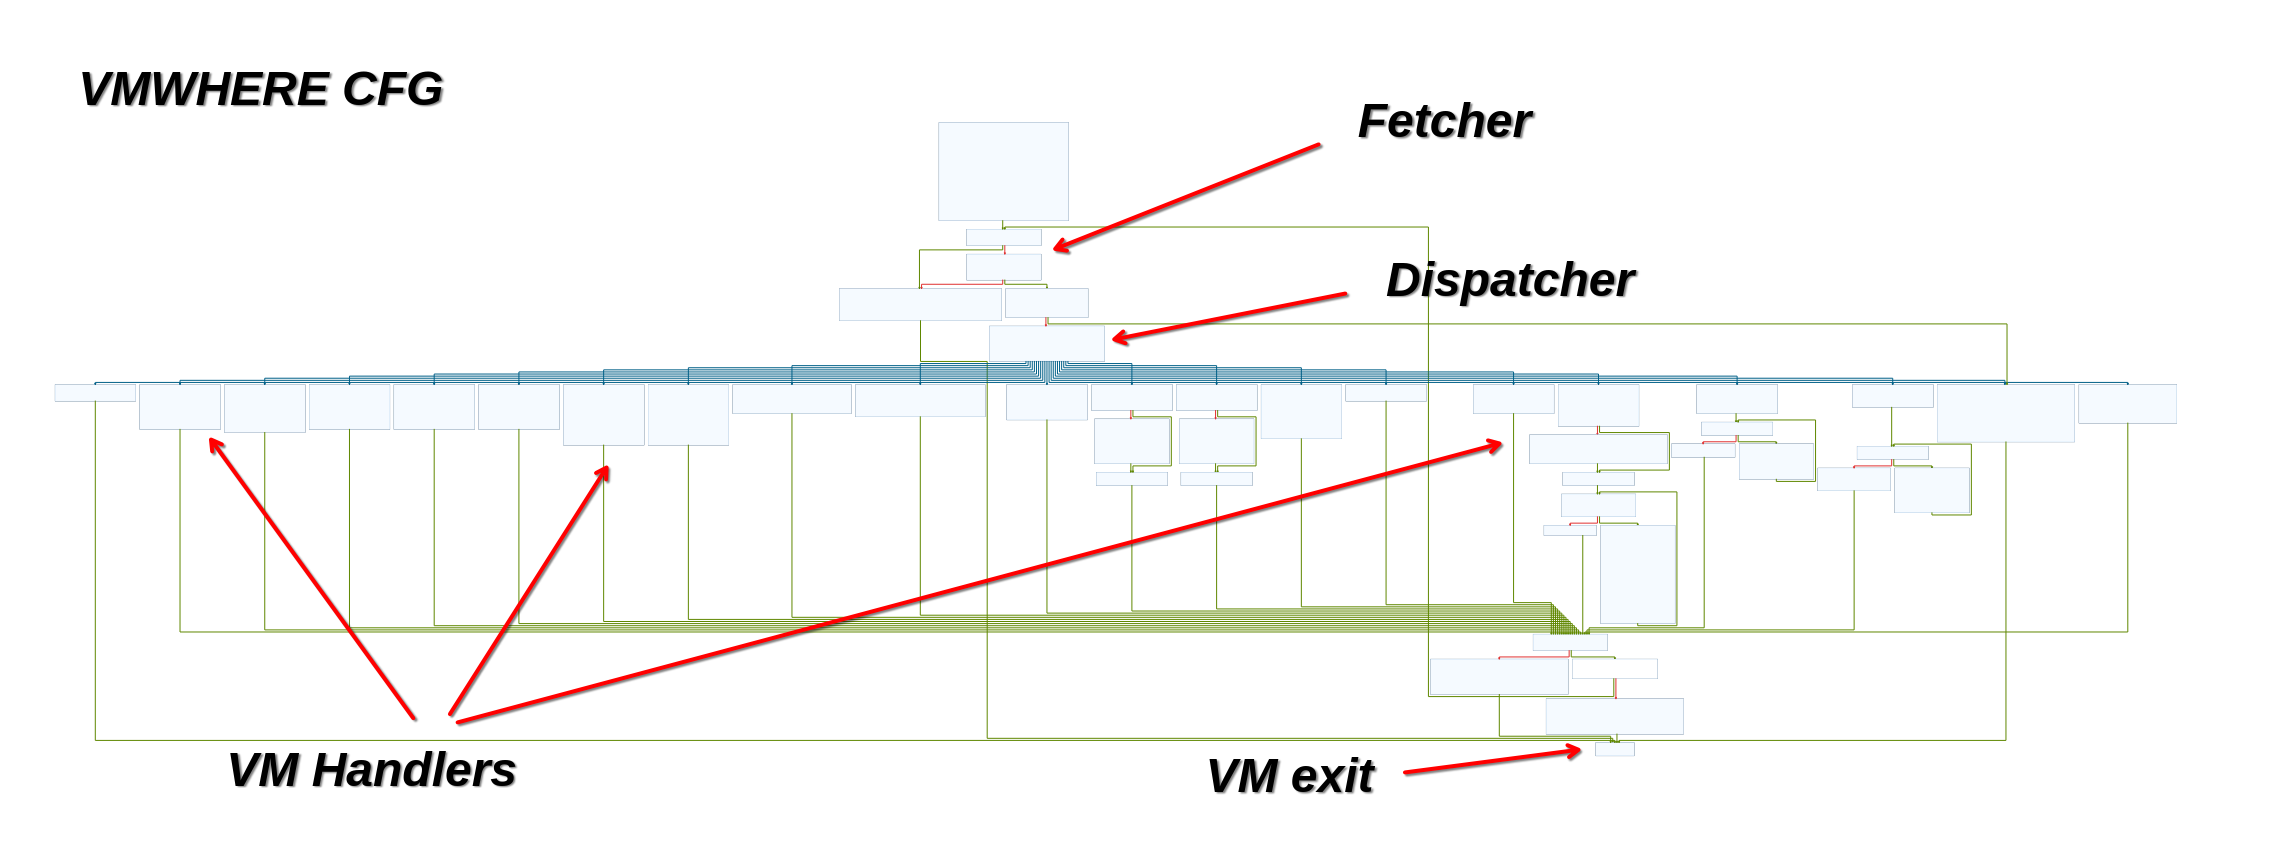
\includegraphics[width=\textwidth]{./images/cfg_vmwhere}
    \caption{\gls{CFG} of the \cc{vmwhere} \gls{VM} interpretor. The major components, such as the instruction fetcher, the dispatcher, \gls{VM} handers, as well as the \gls{VM} exit are clearly labelled. The image is generated with the help of the Cutter \gls{RE} tool \cite{cutter}.}
    \label{fig:cfg_vmwhere}
\end{figure}

We first consult the \gls{CFG} view in order to identify the relevant components of the bytecode interpretor. We are looking for a generic and well known structure of a \gls{VM}, which consists of: a \gls{VM} entry where the context switch from \emph{normal} execution to virtualised execution takes place, a fetch-decode-dispatch loop which extracts each encoded operation from the bytecode, processes it, passes execution to the corresponding opcode handler function, and then continues with the next iteration, or exists, and a \gls{VM} exit, which restores the state and passes control back to \emph{normal} execution. We identify these components in the high level overview, as we can see in Figure \ref{fig:cfg_vmwhere}, for one of the binaries. We can visibly see the individual handlers, as well as there being some handler functions which are more shallow in complexity (mainly on the left side of the \gls{CFG}), and some that are visibly more complex than others (mainly on the right side of the \gls{CFG}). 

\begin{lstlisting}[language=c, label={lst:switch_vmwhere}, caption={Decompilation section of the \cc{vmwhere} dispatcher, after variable renaming and retyping. We notice the implementation of the \cc{add}, \cc{jlz} and \cc{push_top} instructions.}]
switch(*IP) {
case 0:
    return 0;
case 1:
                        /* add */
    SP[-2] = SP[-2] + SP[-1];
    SP = SP + -1;
    IP = rip_next;
    break; //...
case 0xb:
                        /* jlz bb */
    if ((char)SP[-1] < 0) {
    rip_next = rip_next + CONCAT11(*rip_next,IP[2]);
    }
    IP = rip_next;
    IP = IP + 2;
    break; //...
case 0xf:
                        /* push top() */
    *SP = SP[-1];
    SP = SP + 1;
    IP = rip_next;
    break;
}
\end{lstlisting}

The \emph{dispatch} tree is clearly visible in the case of the \cc{vmwhere} challenge, because the dispatching is done via direct jumps. In fact, the Ghidra decompilation shows a big \cc{switch} statement which decodes every opcode individually, as can be seen in Listing \ref{lst:switch_vmwhere}. In the of the \cc{vmcastle} binary, the handlers are not visible in the \gls{CFG} at all, because the dispatching mechanism employed is different. Each handler routine is accessed via an indirect jump, more precisely a call instruction on the \cc{RDX} register. The \cc{RDX} register indexes into a function dispatch table, based on the current opcode. Listing \ref{indirect_call_vmcastle} contains the relevant disassembled code for this example, which is a form of obfuscation.

\begin{lstlisting}[label={lst:indirect_call_vmcastle}, caption={x86\_64 disassembly of the \cc{vmcastle} dispatcher. The function handler corresponding to the current opcode is indirectly called through the register \cc{RDX}.}]
...
0x10281c      LEA       RDX, [RAX*0x8]
0x102824      LEA       RAX, [G_MNEMONICS]
        // Compute offset in the dispatch table
0x10282b      MOV       RDX, qword ptr [RDX + RAX*0x1] 
0x10282f      MOVSX     EAX, byte ptr [RBP + -0x11a]
0x102836      MOV       EDI, EAX
        // Call the corresponding handler function
0x102838      CALL      RDX  
...
\end{lstlisting}

We are also interested in the internal structures of the \gls{VM}, namely, the
registers used, the stack, the memory addressing scheme, calling convention,
etc. The most important registers to look out for are the virtual \gls{IP} and
the virtual \gls{SP}, which we quickly identify. We also notice the location of
the stack and the fact that it \emph{grows} upwards in both cases. A notable
distinction between the \cc{vmwhere} and the \cc{vmcastle} architectures is that
the former performs all its operations directly on the stack, while the latter
uses 4 extra registers for its operations. This is clearly highlighted in
Listings \ref{lst:add_vmwhere} and \ref{lst:add_vmcastle}, where the
implementation of corresponding \cc{add} operations is displayed. The way
operations are performed and how data moves around inside the \gls{VM} is
important information which we need throughout the rest of the analysis.

\begin{multicols}{2}
    \begin{lstlisting}[language=c, label={lst:add_vmwhere}, caption={Stack-based implementation of a simple \cc{add} instruction in the \cc{vmwhere} architecture.}]
SP[-2] = SP[-2] + SP[-1];
SP = SP + -1;
IP = rip_next;
break;
\end{lstlisting}
\columnbreak
\begin{lstlisting}[language=c, label={lst:add_vmcastle}, caption={Register-based implementation of a simple \cc{add} instruction in the \cc{vmcastle} architecture.}]
MEM.AC = MEM.R2 + MEM.R1;
return;
\end{lstlisting}
\end{multicols}

After getting a high-level overview, we continue the analysis with a mix of static and dynamic analysis, in order to better understand the details of each of \gls{VM} handler function. Moreover, we will discuss next about a more unusual technique, which can be very useful in such scenarios.

\subsection{Automatic handler analysis using Miasm}
\label{sec:miasm}

% There is a cool paper that does this, from 2018. cite it. and also mention that @ in miasm IR stands for derefferencing. and also that the output is miasm IR.

This is a short digression from the main topic, to discuss a technique which could prove very useful when analysing obfuscated code in general. We have seen this technique mentioned in multiple places including the Miasm blog in an article about reverse engineering the ZeusVM malware \cite{zeusvm_miasm}, as well as in multiple workshops by Tim Blazytko, such as \cite{tim_miasm}. It involves using Miasm \cite{miasm}, a powerful reverse engineering framework, in order to automatically parse all \gls{VM} handlers and output their semantics in a clear and structured way. 

Miasm, just like angr, at their core, are just emulators, and will function just like a normal emulator when computing strictly on concrete (non-symbolic) data. The beauty happens when we introduce and allow symbolic variables to exist in the state. In that case, by executing several blocks of code, we register the state change across instructions, through the symbolic variables. As such, from the high-level static analysis performed previously, we collect the addresses of each individual instruction handlers and execute them symbolically. In order to limit the scope, we also identify the address where the execution loops back to the start of the dispatch loop: \cc{001018fd | eb 7b | JMP | DISPATCH_LOOP}. Let's take for example a more interesting handler from the \cc{vmwhere} \gls{VM}, in particular the handler number $17$, and execute it symbolically. We can see a partial result in Listing \ref{lst:miasm0}. 

\begin{lstlisting}[label={lst:miasm0}, caption={Partial result of symbolically executing a function handler in Miasm. One will notice the state change in core registers such as \cc{RDX}, flag changes, as well as changes in memory.}]
IRDst = 0x18CF
cf = ((((@64[RBP + 0xFFFFFFFFFFFFFFF0] + 0x7) ^ (@64[RBP + 0xFFFFFFFFFFFFFFF0] + 0xFFFFFFFFFFFFFFFF)) & ((@64[RBP + 0xFFFFFFFFFFFFFFF0] + 0xFFFFFFFFFFFFFFFF) ^ 0xFFFFFFFFFFFFFFF7)) ^ (@64[RBP + 0xFFFFFFFFFFFFFFF0] + 0x7) ^ (@64[RBP + 0xFFFFFFFFFFFFFFF0] + 0xFFFFFFFFFFFFFFFF) ^ 0x8)[63:64]
zf = @64[RBP + 0xFFFFFFFFFFFFFFF0] == 0xFFFFFFFFFFFFFFF9
RDX = {{@8[@64[RBP + 0xFFFFFFFFFFFFFFF0] + 0xFFFFFFFFFFFFFFFF] >> 0x7 0 8, 0x0 8 32} & 0x1 0 32, 0x0 32 64}
RIP = 0x18CF
...
@8[@64[RBP + 0xFFFFFFFFFFFFFFF0] + 0x4] = (@8[@64[RBP + 0xFFFFFFFFFFFFFFF0] + 0xFFFFFFFFFFFFFFFF] >> 0x5) & 0x1
@8[@64[RBP + 0xFFFFFFFFFFFFFFF0] + 0x5] = (@8[@64[RBP + 0xFFFFFFFFFFFFFFF0] + 0xFFFFFFFFFFFFFFFF] >> 0x6) & 0x1
@8[@64[RBP + 0xFFFFFFFFFFFFFFF0] + 0x6] = (@8[@64[RBP + 0xFFFFFFFFFFFFFFF0] + 0xFFFFFFFFFFFFFFFF] >> 0x7) & 0x1
@8[@64[RBP + 0xFFFFFFFFFFFFFFF0] + 0xFFFFFFFFFFFFFFFF] = @8[@64[RBP + 0xFFFFFFFFFFFFFFF0] + 0xFFFFFFFFFFFFFFFF] & 0x1
\end{lstlisting}

% TODO I want to mention that we update the python2 script from zeus, and now it works with python3 

This output is complete, but not very useful in this form for two reasons. Firstly, the output includes changes in flags and other side effects of the mnemonic execution that we are not particularly interested in. Secondly, the data that we are interested in is presented as memory offsets from \cc{RBP}, which are particularly difficult to read. We can tackle both points by ignoring the changes on memory that we are not interested in and by substituting memory addresses that we are interested in with explicit labels. The result of this transformation can be seen in Listing \ref{lst:miasm1}.

\begin{lstlisting}[label={lst:miasm1}, caption={Result of symbolically executing the same function handler as in Listing \ref{lst:miasm0} with some cleanup. We only chose to display the change in relevant registers and memory locations. Additionally, we introduced labels for better clarity.}]
*************** | Mnemonic 17 | addr: 0x17DE | ***************
VM_SP = VM_SP + 0x7
VM_STACK_TOP = VM_STACK_TOP & 0x1
@8[VM_SP] = (VM_STACK_TOP >> 0x1) & 0x1
@8[VM_SP + 0x1] = (VM_STACK_TOP >> 0x2) & 0x1
@8[VM_SP + 0x2] = (VM_STACK_TOP >> 0x3) & 0x1
@8[VM_SP + 0x3] = (VM_STACK_TOP >> 0x4) & 0x1
@8[VM_SP + 0x4] = (VM_STACK_TOP >> 0x5) & 0x1
@8[VM_SP + 0x5] = (VM_STACK_TOP >> 0x6) & 0x1
@8[VM_SP + 0x6] = (VM_STACK_TOP >> 0x7) & 0x1
\end{lstlisting}

With the correct labelling, the comprehension of the handler's behaviour is not that hard to understand any longer. It takes the 1-byte value from the top of the stack, and for each of the bits comprising it, an equivalent bit is pushed onto the stack. For example, if we had the value $[1e]$ on the stack, we would end up, instead, with the following values on the stack $[0, 1, 1, 1, 1, 0, 0, 0]$. We can confirm with fact with the Ghidra decompilation, or with a disassembler, where we will observe a loop which pushes each individual bit from the respective byte, on the stack. 

By studying both the decompiled code and the output from the Miasm we were able to recover the semantics of all the handlers. 

It is important to note, that the true power of this analysis technique is not fully highlighted in this scenario with the two \gls{CTF} challenges, as the samples lack more complex obfuscation. The blog post from Miasm about ZeusVM \cite{zeusvm_miasm} is a better example, because there are considerably more function handlers to analyse, but also, some of them are very similar. This technique can be further used to compare symbolic states, in order to identify what the exact differences between certain handlers are, through a simple difference operation. When dealing with heavier obfuscation, Miasm's symbolic execution engine can deal with techniques such as \emph{constant unfolding}, \emph{dead code}, \emph{pattern based-obfuscation}, by simplifying the mathematical expressions that arise. Even more, in the case of \gls{MBA}, which is one of the most difficult to deal with obfuscation schemes, we can use a msynth \cite{msynth}, a framework built on top of Miasm which can simplify \gls{MBA} expressions, based on one of the most generic and powerful attacks on \gls{MBA}, called QSynth \cite{qsynth}.

\section{Summary of Analysis}

Manual static analysis in Ghidra, as well as symbolic analysis using Miasm, which were previously discussed, are the main techniques which we used in order to reverse engineer the custom \gls{ISA} of the embedded \gls{VM}. We were able to identify the main data types used, the registers, as well as the individual instructions. We were able to identify and understand the implementation of the following instructions: 

\begin{enumerate}
    \item arithmetic and logic operations: We identifies a number of function handlers which perform simple arithmetic operations, resembling instructions such as \cc{add}, \cc{sub}, \cc{xor}, \cc{shl}, \cc{shr}, \cc{mul}, \cc{div}, from well known architectures. The implementations in the two targeted \glspl{VM} are not the same. In the \cc{vmwhere} binary, the operations are computed using strictly values from the top of the stack, while in the case of \cc{vmcastle}, the operations are done via registers.
    \item stack operations: Both \glspl{ISA} have similar implementations of the \cc{push} and \cc{pop} instructions. We could also identify variations where the value of a registers is pushed onto the stack, a value is popped into a register (or not), the popped values is also printed to \cc{stdout}, etc.
    \item conditionals and jumps: We identified function handlers which resemble in behaviour instructions such as \cc{cmp}, \cc{jlz}, \cc{jz}, \cc{jmp}. In the case of \cc{vmwhere}, all conditional checks are made on the value on top of the stack, and the jumps are all \emph{direct}, relying on immediate values as offsets from the current position. In the case of \cc{vmcastle} the implementations are slightly more complex. The \cc{cmp} operation updated the flag register \cc{ac}. Subsequently, a conditional jump will perform an indirect jump based on the \cc{ac} flag, taking the value stored in one of the three other registers  (\cc{r1}, \cc{r2}, \cc{r3}) as an offset.
    \item \gls{syscall}: In both cases we identified handlers which perform reads and writes. Both operations result in a context switch to the kernel as a result of \glspl{syscall} in the host \gls{OS}. Their implementation is straight forward. In the case of \cc{vmwhere} the value is read/wrote onto/from the stack, whilst in the \cc{vmcastle} case, data is read and wrote into and from registers. Since we are dealing with \glspl{syscall}, in the angr plugin implementation that follows, special measures will have to be taken for correctly implementing these instructions.
    \item \cc{nop} and exits: In both cases we identified \cc{exit} instructions which just simply signal to the embedded interpreter that the execution of the bytecode should cease and context should be switched back to the core execution. In the case of \cc{vmcastle} we also encountered 101 entries in the dispatch table, which all point to the same instruction handler. The implementation of this instruction does nothing, and constitutes the equivalent of a \cc{nop}.
    \item adhoc and complex instructions: In both cases, but especially in the case of \cc{vmwhere}, we identified function handlers that do not resemble any well known instructions from common architectures, but rather a combination of multiple instructions, leading to a more complex set of transformations which are applied to the state of the program. In the case of \cc{vmwhere} there are two conditional arithmetic operations applied to the top of the stack: a \cc{shl} and an \cc{add} operation which will be applied or not with an argument of $1$, based on an immediate value. In the case of \cc{vmwhere}, the handlers which stand out are handler number $17$, also mentioned in Section \ref{sec:miasm}, and handler number $18$, which performs the reverse operation. Moreover, handler number $16$ reverses the order of the elements on the stack in a given range, specified through an immediate value.
\end{enumerate} 

Other relevant information is the size of the stack, which in both cases is of $4096$ bytes. An unusual piece of information, is that in the case of \cc{vmcastle}, the stack is cyclic, meaning that after pushing $4096$ elements on the stack, the $4097$th will override the first element. All the information acquired during this stage is crucial for the proper implementation of the \cc{angr} plugin.

\section{Building an angr architecture plugin}

In this section, we will cover \cc{angr} \cite{angr}, a popular binary analysis framework, which has been growing in popularity in the security scene. It is built in python and designed to be modular and extensible. Thus, each of its modules can be easily extended. Figure \ref{fig:angr} clearly depicts angr's components and the way in which those interact. Our goal is to be able to write a simple angr program (such as Listing \ref{lst:angr_ex}) which loads a binary file containing bytecode written for one of our custom architectures. We expect that to have angr be able to load it, parse it, run analysis tools on it and symbolically execute it. We essentially want angr to treat our binary file just like any other binary file based on a common architecture, such as \cc{x86_64}. We will now go over the components which we extended in our plugins. We took a lot of inspiration from a tutorial on how to build an angr plugin for \gls{BF}, and other examples showcased by the angr team on their Github page \cite{angr_tut}.

% TODO should mention smth about claripy
\begin{figure}
    \centering
    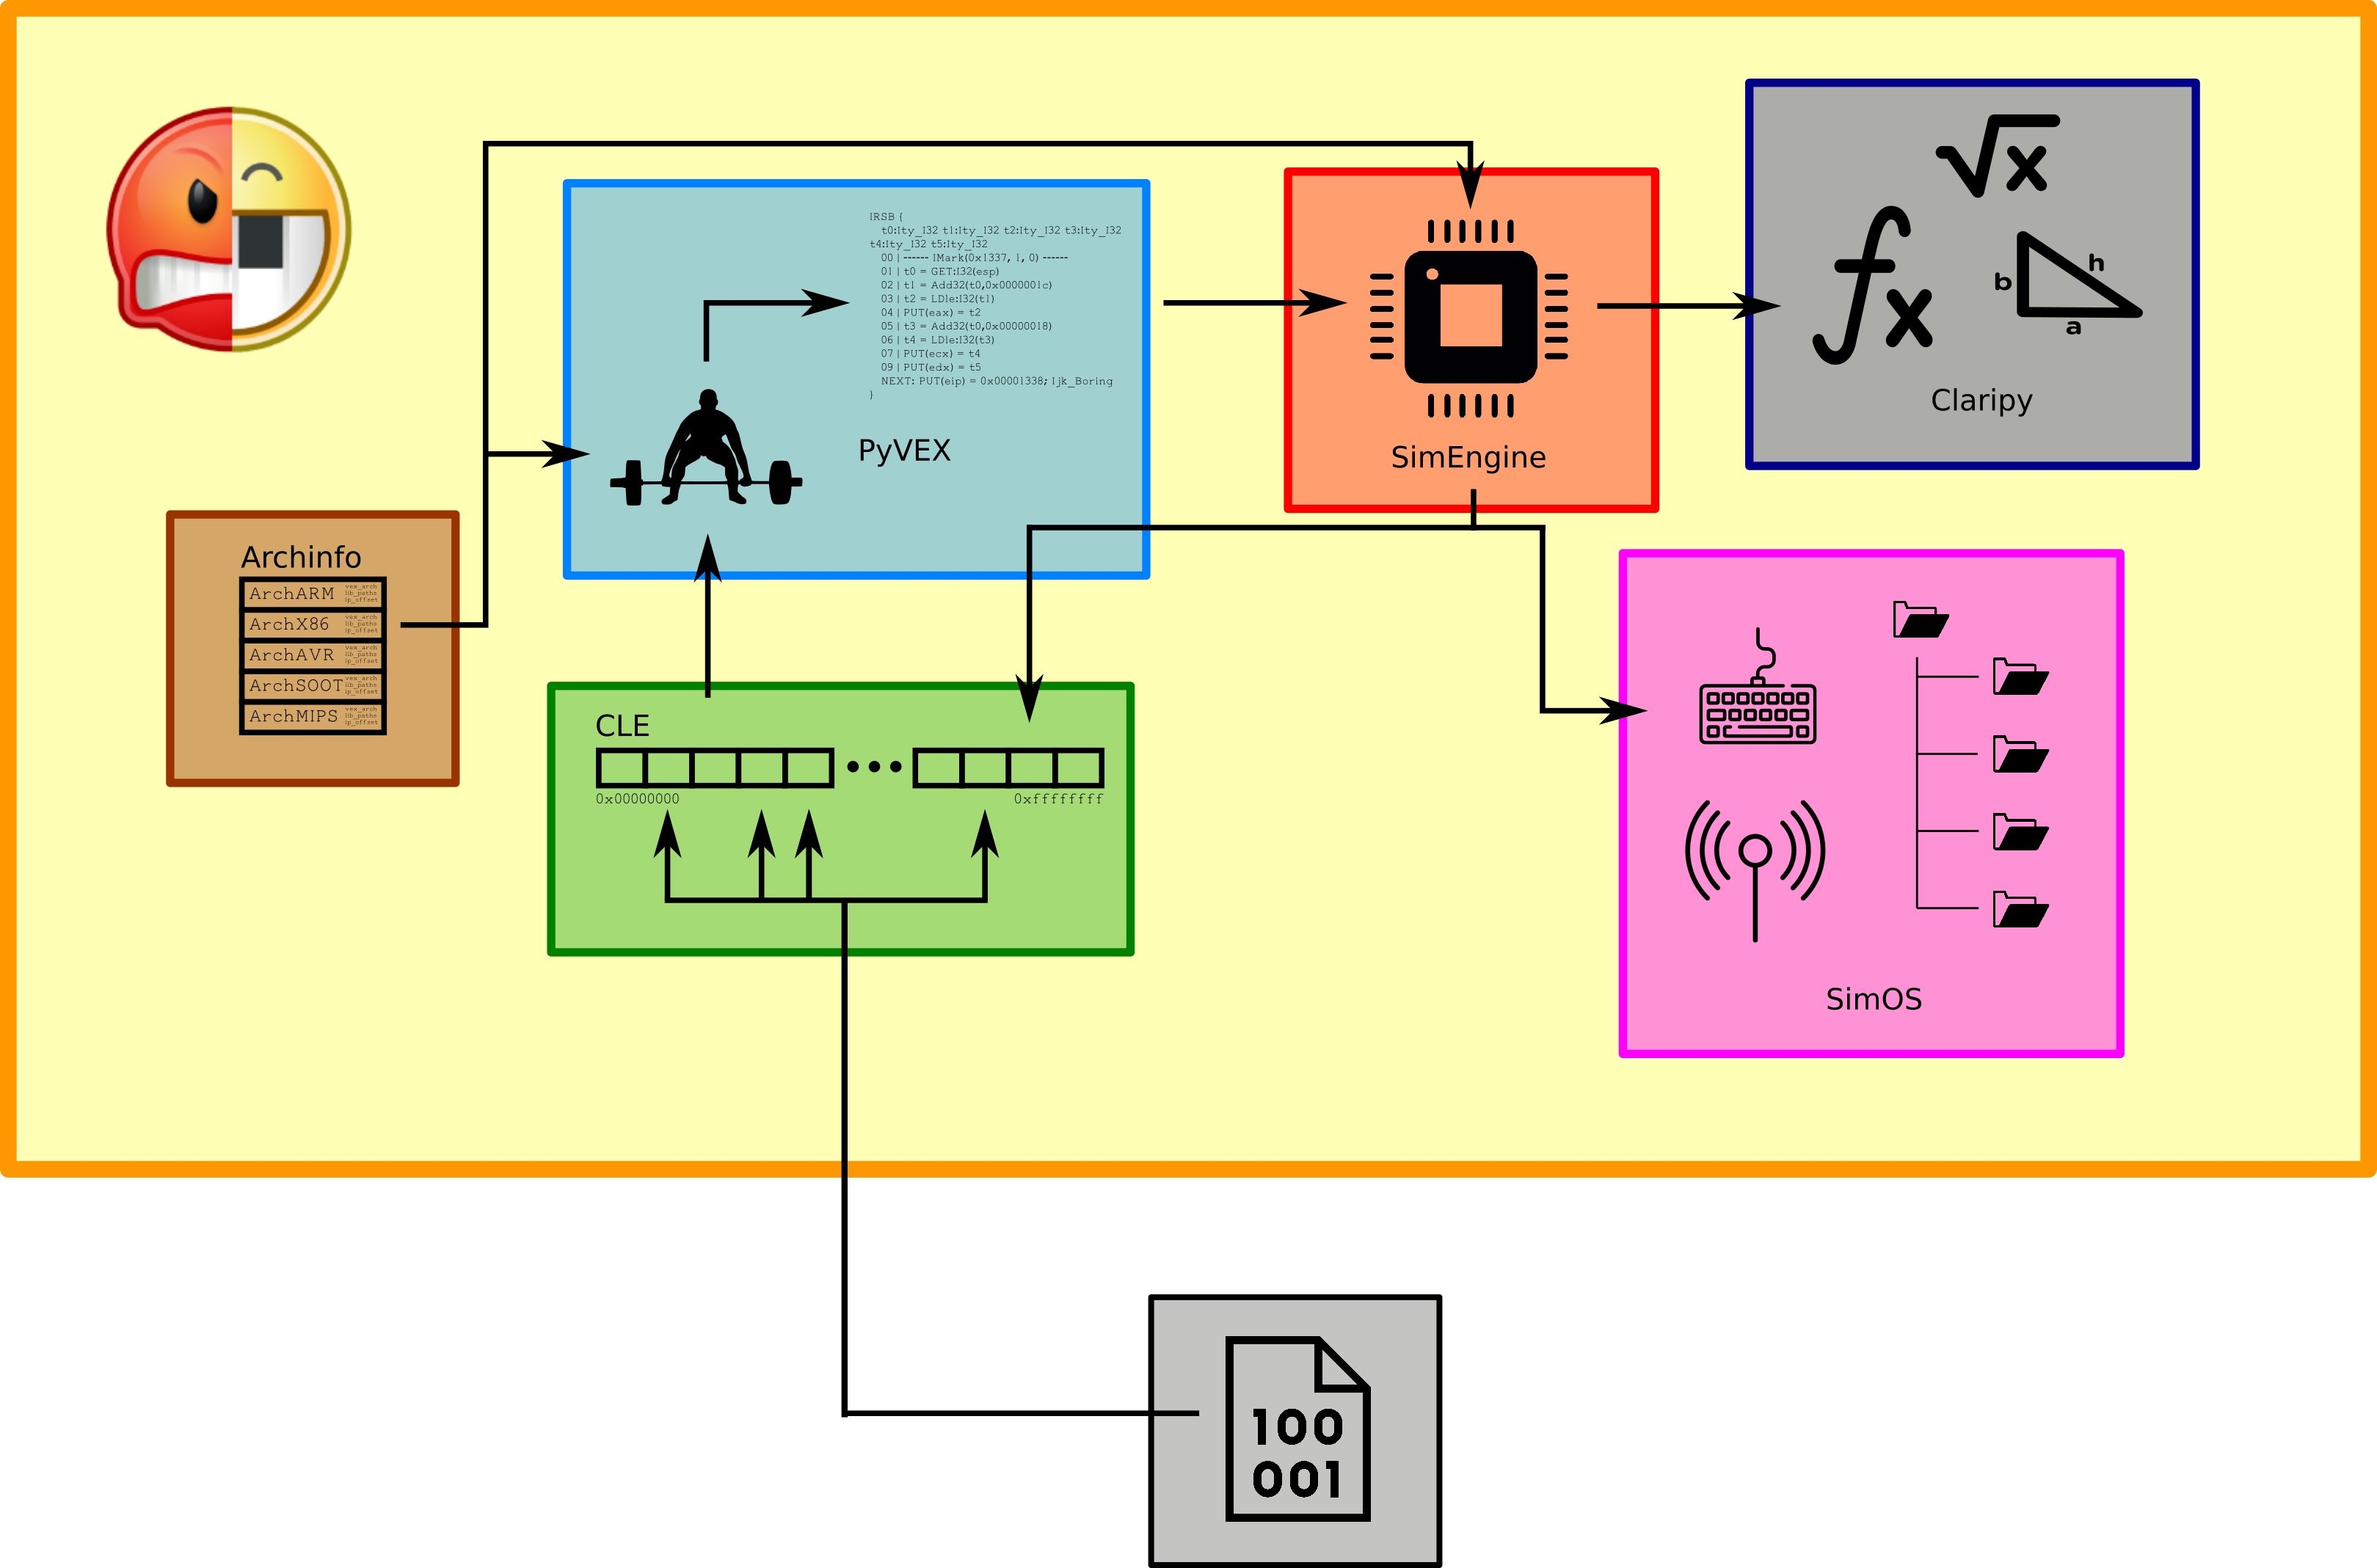
\includegraphics[width=0.9\textwidth]{./images/angr.png}
    \caption{TODO}
    \label{fig:angr}
\end{figure}

\begin{lstlisting}[language=python, label={lst:angr_ex}, caption={A minimal angr code sample. We load a program into \cc{p}, create a simulation manager, symbolically execute the program until we reach the desired address \cc{0xcafebabe}, and finally print the input which determined this execution path.}]
import angr
p = angr.Project("program") # program for our custom architecture @$ \label{line:project} $@
sm = p.factory.simulation_manager()
sm.step(until=lambda s: s.addr == 0xcafebabe) # symbolic execution
print(f'input: {sm.active[0].posix.dumps(0)}') # retrieving the input
\end{lstlisting}

\subsection{A new entry in the Arch database}

\cc{Arch}, short for \cc{Archinfo}, is an architecture database, where each entry holds all structural details regarding an architecture. To exemplify, in our case, this entailed the list of registers, the bit-width, endian-ness, alignment and name. Listing \ref{lst:angr_arch} shows how we inherit from the \cc{Arch} class and add relevant information about our particular architecture, in this case, \cc{vmwhere}. Line \ref{line:reg_arch} from the same code Listing, which contains the \cc{register_arch} function call, is very important, because it \emph{let angr know} that a new architecture has been added, which should be considered during program loading. One will notice two registers which we did not mention before: \cc{sysnum} and \cc{ip_at_syscall}. These two registers are not part of the architecture, but are relevant in angr's protocol for \glspl{syscall}. As a matter of fact, \cc{bp} is also not part of the architecture, but we added it for convenience and easier debugging. Although it is not a lot, this information is a crucial part of our package.

\begin{lstlisting}[language=python, label={lst:angr_arch}, caption={TODO}]
class ArchVMWHERE(Arch):
    bits = 64
    instruction_alignment = 1
    memory_endness = Endness.LE
    name = "vmwhere"

    register_list = [
        Register(name="ip", size=8, vex_offset=0, alias_names=['pc'],),
        Register(name="bp", size=8, vex_offset=8,),
        Register(name="sp", size=8, vex_offset=16,),
        Register(name="sysnum", size=8, vex_offset=24,),
        Register(name="ip_at_syscall", size=8, vex_offset=32,),
    ]

register_arch(['vmwhere|VMWHERE'], 64, Endness.LE, ArchVMWHERE) @$\label{line:reg_arch}$@
\end{lstlisting}

\subsection{Extending the Loader}

When we first load a program in \cc{angr}, by default it will try to determine the architecture of the file, and find an instance of an \cc{Arch} class which matches that guess (see Line \ref{line:project} in Listing \ref{angr_ex}). The component which takes care of this step is the loader: \gls{CLE}. In order to build a custom loader for our architecture we must inherit from the \cc{Blob} class and add some relevant information on how we want the binary file to be loaded: the number of bytes which should be skipped from the beginning (offset), where the entry point of the program is, and the base address. Then, we must also override the \cc{is_compatible} method, which checks if an input binary file matches the expected architecture. In our implementation artificially introduced a 3-bytes header into the bytecode for easier identification, but our experiments show that this it is not necessary. If we register only one custom architecture during analysis, all the loaders for the well known architectures will fail, and, as a consequence, our loader will be selected. However, in the unlikely scenario in which we would instrument simultaneously two different programs, with different custom architectures, we would have to make sure that we take the necessary measures for each of them to be correctly identified. In the end, we register the new loader with the \gls{CLE} backend.

\subsection{Building a Lifter}

angr is a multiplatform binary analysis platform and can be easily extend to also support other architectures. The main reason behind this powerful mode of operation is the following: angr's every type of analysis that is performed through angr is done on an \gls{IR} called VEX. In fact, VEX is the same \gls{IR} used by Valgrind, another binary analysis platform which specialises in detecting memory corruption issues, profiling, and others \cite{valgrind}. Thus, in order to instrument code for a custom architecture, we do not need to implement a new custom analysis engine, but only to provide a translation layer between the bytecode we provide and the VEX \gls{IR}. This translation layer is called a lifter, because it \emph{lifts} the bytecode into a higher level representation. angr provides a framework called \cc{gymrat}, which simplifies the process of building a lifter, which is a further abstraction over \cc{pyvex} -- a pythonic interface over the VEX \gls{IR} objects.

In order to build a lifter for a custom architecture we must define the format for syntax and semantics of each instruction. Typically, the syntax is given by the length of the instruction, a fixed \emph{magic number} which identifies it, called the opcode, and the arguments. Then, in order to express the semantics of the instructions, we have to describe the state change that the execution of the instruction would produce during execution, by utilising the primitives provided through the \cc{pyvex} framework. These primitives consist of operations which enable using immediate values in the form of constants, reading/writing data from/to pointers, reading/writing data from/to memory, and jumping. These primitives are sufficient for expressing the vast majority of program logic, but are sometimes lacking, as we will discuss in a later section \ref{sec:shortcomings}.

\begin{lstlisting}[language=python, label={lst:instruction}, caption={TODO}]
class Instruction_JZ(Instruction):
    bin_format = '00001100xxxxxxxxxxxxxxxx'
    name = 'jz'

    def compute_result(self, *args):
        jump_offset = int(self.data['x'], 2)
        dst = self.constant(self.addr + self.bitwidth // 8 + jump_offset, Type.int_16).signed @$ \label{line:instruction0} $@

        sp = self.get(SP_REG, PTR_TYPE) @$ \label{line:instruction1} $@
        top = self.load(sp - 1, STACK_ENTRY_TYPE).signed @$ \label{line:instruction2} $@
        zero = self.constant(0, STACK_ENTRY_TYPE)

        self.jump(top == zero, dst)  @$ \label{line:instruction3} $@
\end{lstlisting}

To give an example, let us consider an implementation of a \cc{jz} (jump when zero) instruction as seen in Listing \ref{lst:instruction}. We define a class, which inherits the base \cc{Instruction} class exposed by \cc{pyvex}. We define the syntax as a binary string in \cc{bin_format}. The first eight bits represent the opcode (number $12$), and 16 that follow represent an immediate value of two bytes. We mark it with 16 \cc{x} characters, firstly in order to represent the sequence of bits as a wildcard, and secondly in order to more easily retrieve the data from the sequence during the lifting process. The logic of the instruction is given by overriding the \cc{computer_result} method. We start by retrieving the jump offset from the immediate value \cc{x}, we compute the destination address, on Line \ref{line:instruction0}, load the value in the stack pointer, on Line \ref{line:instruction1}, load the value on top of the stack in Line \ref{line:instruction2} and finally perform a conditional jump to the computed address, when the value on top of the stack is equal with the constant value zero, on Line \ref{line:instruction3}.

Similarly, we provide an implementation for the rest of the instructions. To finalize the lifter, we define a class which inherits from the base class \cc{GymratLifter}, and give it a list containing all possible instructions that might be encountered when analysing a binary file for our custom architecture, in the exact order that they should be parsed -- meaning that more generic instruction should be left at the end. We then register the new lifter with angr.

\subsection{SimOS}

The last component which we must extend is \cc{SimOS}, an abstraction layer for the \gls{OS}. An instance of a SimOS class is created based on the architecture identified by the loader. It exposes simplified symbolic abstractions of \gls{OS}-specific entities, such as files or network components, \glspl{syscall}, or common standard library functions in the form of \cc{SymProcedures} \cite{angr_tut}. The SimOS component exists to eliminate the very complex task of interpreting complex code that is not directly related to the main target of the analysis. As also stated by the angr team, ``symbolically executing libc itself is, to say the least, insanely painful'' \cite{angr_tut}. 

In our case, we wrote a minimal SimOS implementation in order to deal with the \cc{read} and \cc{write} handlers. We implemented two SymProcedures, one for each of the \glspl{syscall}. An example implementation of the \cc{write} \gls{syscall} can be seen in Listing \ref{lst:simproc}. We created a class, which inherits from \cc{SimProcedure}, and overridden the \cc{run} method. The parameter \cc{sp} is used as a result of the calling convention which we also had to define as part of the same extension.

\begin{lstlisting}[language=python, label={lst:simproc}, caption={TODO}]
class WriteByte(SimProcedure):
    def run(self, sp):
        # Write a byte to stdout
        self.state.posix.fd[1].write(sp, 1) 
\end{lstlisting}

\section{Plugin Generation - arch-genesis}

After we writing the necessary extensions, we grouped them in a python package. By importing the newly created package (\cc{from vmwhere import *}), the example provided in Listing \ref{lst:angr_ex} will function according to our expectations. Even more, all of angr's analyses will function accordingly, because all of these operate on VEX, which can be extracted from any bytecode wrote for the respective \gls{VM}. Our work is, however, not nearly completed. Despite the high level abstractions that \cc{angr} exposes, writing such a custom architecture plugin still requires a considerable amount of effort to be spent on implementation details that are not related to the analysis of our target bytecode.

To mitigate this, we propose \cc{arch-genesis}, a tool which generates all the necessary boilerplate code necessary for a plugin, so that the analyst can focus only on writing code for the relevant parts of the engine: the logic for the instructions in the lifter, and the necessary SymProcedures. The generator is built in python, using the jinja2 \cite{jinja} template engine. All relevant information regarding the \gls{VM}, that is relevant for generating the plugin (eg. name, registers, endian-ness, list of instructions, etc.) is provided via a carefully and intuitively structured config file. We chose \cc{TOML} \cite{toml} as the format of choice for the config files, because of its ease of writing compared to \cc{json} and its lack of ambiguity compared to \cc{YAML}. Listing \ref{lst:config} contains a section of the config file we used in order to generate the \cc{vmcastle} plugin.

\begin{lstlisting}[label={lst:config}, caption={TODO}]
...
[lifter.opcodes.stack_top_itshl]
bin_format = [ 115, ['r', 8] ]

[lifter.opcodes.stack_top_itadd]
bin_format = [ 116, ['r', 8] ]

[loader]
offset = 0
entry_point = 0
base_addr = 0x000000
header = ''

[simos]
syscall_args = [ 'reg_no' ]
return_addr = [ 'ip_at_syscall', 8 ]
syscall_addr_alignment = 8

[[simos.syscalls]]
syscall_no = 0
name = 'ReadByte'
...
\end{lstlisting}

\subsection{What about a Disassembler?}

One of the most important aspects of binary analysis is being able to read code in order to understand what it does, as we have described for instance in Section \ref{static_ghidra}. Using a disassembler is still essential, even when attempting automatic analysis with a tool such as angr, in order to determine relevant simple blocks and determine strategies of guiding execution. As such, at the very least, we would need a disassembler for the bytecode that we are analysing. When analysing \emph{classic} programs, we can check out the disassembly of the machine code through the well integrated capstone disassembly framework \cite{capstone}. We could theoretically write a capstone module for our custom architecture, but to achieve such a thing would require an unreasonable amount of effort, which is outside the scope of this work.

\begin{lstlisting}[label={lst:disass}, caption={TODO}]
0x17c4:  push_imm b'?'
0x17c6:  pop_reg ac
0x17c8:  print_reg ac
0x17ca:  push_imm b'\xff'
0x17cc:  pop_reg r3
0x17ce:  push_imm b'\n'
0x17d0:  pop_reg r2
0x17d2:  read_reg r1
0x17d4:  push_reg r1 | push the value in the register on the stack @$ \label{line:desc} $@
0x17d6:  cmp  | compare R1 and R2; set AC
0x17d8:  push_imm b'\xf4'
0x17da:  pop_reg r1
0x17dc:  push_imm b'\x00'
0x17de:  pop_reg r2
0x17e0:  push_imm b'\xf4'
0x17e2:  pop_reg r3
0x17e4:  jmp_cond  | jump with reg offset, based on AC | AC < 0: +R1 | AC == 0: +R2 | AC > 0: +R3
0x17e6:  pop_reg r2
0x17e8:  pop_reg r2
0x17ea:  push_imm b'\t'
0x17ec:  pop_reg r1
0x17ee:  add  | ac = r1 + r2
\end{lstlisting}

Luckily, there is enough information available to the lifer in order to also perform disassembly of the bytecode. In fact, the angr team took care of this: there is \emph{hidden} functionality for disassembly, which we were able to extend and customize. Thus, the \cc{arch-genesis} program will generate a disassembly executable, which we can run with any file containing architecture-specific bytecode as input, and will output its corresponding disassembly. An example disassembly sample can be inspected in Listing \ref{lst:disass}. As we can see, for example one Line \ref{line:desc}, the disassembly can be enriched with descriptions of the instruction behaviour, or by changing the formatting of the respective output. All of these enrichments can easily be done from the previously mentioned \cc{.toml} config file.

\section{Further Analysis}

While working with the disassembler and inspecting the implementation of the \cc{gymrat} lifter, we had the idea of also building a \gls{CFG} generator. This might seem strange, knowing that angr has \gls{CFG} building capabilities. In fact, these analyses work, but our goal was to create a visulisation in the \cc{.dot} format and transforming angr's output into dot is not a trivial task. Even more, we were interested in also having the disassembly included in the graph, which would have added another layer of complexity, since the system we were working on for acquiring the disassembly is not fully integrated with the main analyses. Considering the fact that the \cc{vmwhere} \gls{VM} is only capable of performing direct jumps, we wrote a custom \gls{CFG} building algorithm, using common graph theory techniques. The result can be see in Figure \ref{fig:cfg_bytecode}.

\begin{figure}[h]
    \centering
    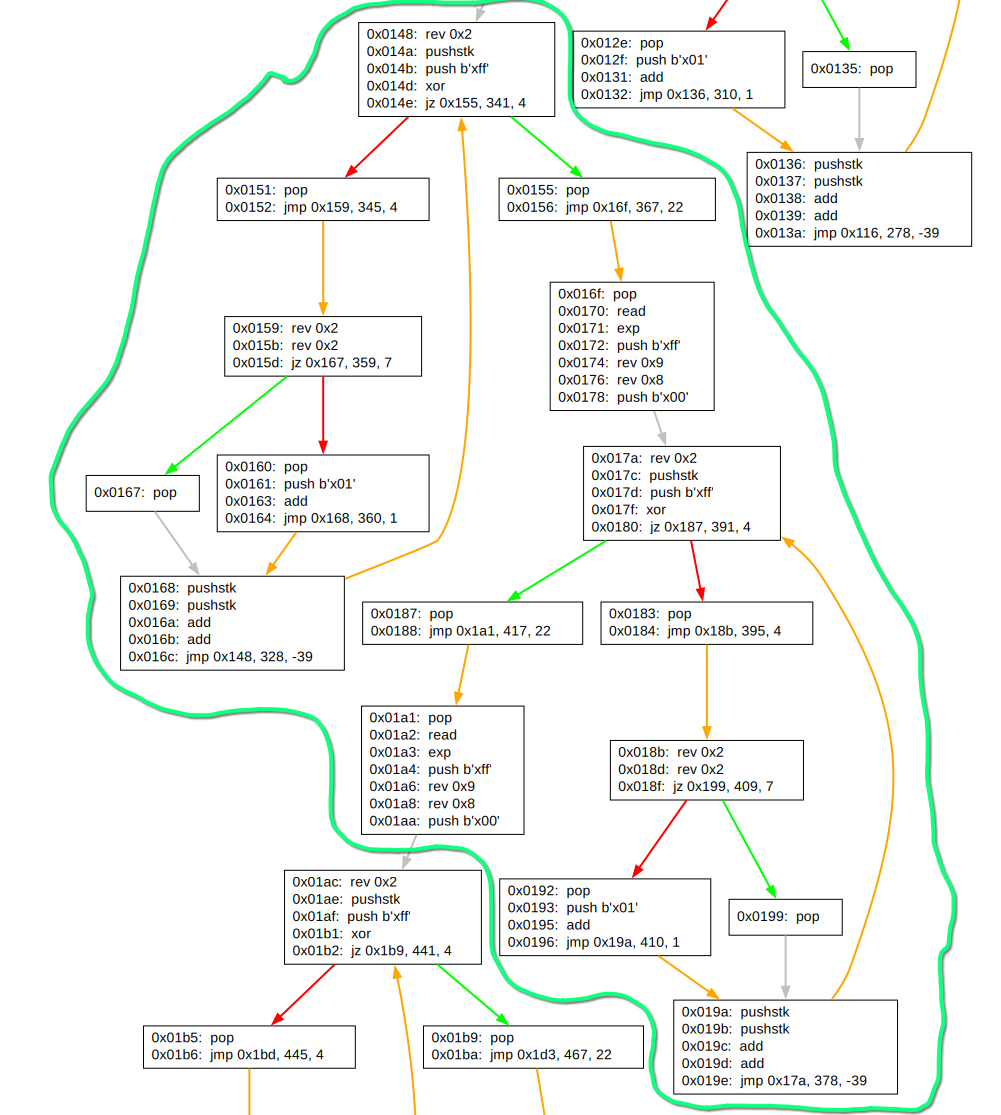
\includegraphics[width=.8\textwidth]{./images/cfg}
    \caption{TODO}
    \label{fig:cfg_bytecode}
\end{figure}

The section circled in green represents a sequence of operations on stack data, which repeats multiple times in the binary. In fact, this corresponds to a form of obfuscation, commonly known as \emph{function inlining}, which we mentioned in Section \ref{TODO}. Visualising the \gls{CFG} clearly helps in identifying this kind of obfuscation, as well as in better understanding the flow of information and how the state of the program changes during execution. Building a \gls{CFG} is however, generally not a trivial task and depends directly on the difficulty of computing jump targets. Because of indirect jumps, we weren't able to apply the same strategy for the \cc{vmcastly} binary.

\subsection{Solving the Challenges}

\subsubsection{VMWHERE}

Static analysis on the disassembly, in conjunction with the \gls{CFG} enabled us to identify the previously mentioned inlined function, which takes a byte of data from \cc{stdin}, and transforms it through a series of operations. We are not particularly interested in what the exact operatins are, because we can symbolically execute them in angr. We are rather interested in how the result is used. The result of each round of computations is stored on the \gls{VM}'s stack. Listing \ref{lst:vmwhere_check} shows another sequence of operations that repeatedly takes place at the end of the program. Being on the shorter side, it is not so difficult to understand that it takes exactly one value from the top of the stack, performs a $xor$ logical operation on it with the byte \cc{\xZZ}, and then performs an $or$ logical operation on the result, with the value at the bottom of the stack, which is initially $0$.

\begin{lstlisting}[label={lst:vmwhere_check}, caption={TODO}]
0x0972:  push b'\xZZ' @$ \label{line:vmwhere_check_imm}$@
0x0974:  xor
0x0975:  rev (sizeof(stack) - 1)
0x0977:  rev (sizeof(stack))
0x0979:  or
0x097a:  rev (sizeof(stack) - 1)
0x097c:  rev (sizeof(stack))
\end{lstlisting}

We are dealing with a \emph{crackme} type of program. What is does is that it accepts an input, performs a series of checks on it, and returns if the input string was accepted or not. Our goal is to find a correct input that bypasses the checker. In this case, the final check that we are interested in, can be found at the very end of the bytecode: \cc{0x0b9a:  jz 0xba0, 2976, 3}. After performing all the rounds which resemble Listing \ref{lst:vmwhere_check}, the only value left on the stack, which is the bottom of the stack, is checked to be equal to zero. The response is considered correct if that check passes. We can extrapolate, and understand that each result of the computation we observed in the \gls{CFG} \ref{fig:cfg_bytecode} is checked for equality against the immediate value from Line \ref{line:vmwhere_check_imm} in the previously mentioned code Listing. By symbolically executing the inlined function, giving it as input a symbolic value, and finally constraining the output to be equal to the immediate value \cc{\xZZ} from Line \ref{line:vmwhere_check_imm}, we will obtain the corresponding input byte that would produce the respective output. We automated this process in angr in repeated it for each of the identified constants in the bytecode in order to recover full secret. %The desired input is: \cc{uiuctf{b4s3_3_1s_b4s3d_just_l1k3_vm_r3v3rs1n@g}

\subsubsection{VMCASTLE}

The second challenge is also a \emph{crackme}. It is, however, a lot more difficult to statically analyse. The bytecode itself is obfuscated with techniques such as \emph{function inlining}, \emph{dead code inserting}, \emph{constant unfolding}, etc. We can bypass these obfuscation techniques, by executing the code symbolically with angr, using our plugin for \cc{vmcastle}. We can only needed needed a small, but crucial, amount of information before automating the whole cracking process:

\begin{enumerate}
    \item In this case, the whole secret is read at once. We found out that it is stored on the stack, and the exact address in the bytecode where input reading ends and the checking process begins. \label{item:one}
    \item We determined a range of addresses that the code would reach if the input was deemed incorrect. \label{item:two}
    \item We determined the first address that would be reached if the input was deemed correct. \label{item:three}
\end{enumerate}

With the above information, we created a symbolic string, inserted it on the stack, and started executing at the address determined in \ref{item:one}. We then start a guided symbolic execute the code in a guided manner: we specifically avoid the range of addresses from \ref{item:two} and try to reach the address from \ref{item:three}. In the end we end up with one state found and many more avoided. At this point we focus our attention on the found state. Its constraint solver has built an expression, which constrains the execution to follow the exact path which lead to the found state. By finding a model which satisfies the constraints, we essentially crack the checker. The full solution can be seen in Annex \ref{TODO}.

\section{Discussion}

We presented how we can reverse engineer and analyse binaries obfuscated with the embedded \gls{VM} technique, by building an angr package which enables an running various analyses techniques directly on the bytecode. We will further discuss our framework choice, difficulties that we encountered, advantages and shortcomings of the technique, as well as future directions.

\subsection{angr vs Miasm}

Throughout this chapter we mainly focused on building an angr plugin, its inner workings, and how it can be used, once finalised, in order to solve two \gls{CTF} challenges. We also discussed automated reverse engineering technique for recovering the semantics of function handlers from the embedded \gls{VM}. For that process, we used another framework capable of symbolic execution, Miasm. A natural question would be: ``why choose one over the other?'' 

A very big difference between angr and Miasm is that angr is in the ease of use and out of the box functionality. angr is, generally, easier to use than Miasm. It exposes higher level abstraction and a lot of functionality our of the box. Moreover, it was designed to be modular, and it was clear very that adding an architecture plugin would enable us to use this big suite of already implemented tools. Miasm, on the other hand, has similar functionality at its core, but doesn't have as much abstraction and needs scaffolding in order to do anything useful with it. Because of that, despite being harder to customize later, we chose angr for the vast array of functionality that it provides by default.

A following question could be: ``why did we not use angr instead of Miasm, to maintain consistency?''. Well, we tried. We quickly realised that angr simply does not offer this functionality in its default tool-set. There exists a conceptually similar analysis named the \emph{Congruency Checker}, which has functionality to compare two states. The output was however rather far from our expectations. In cases such as this one, angr is hard to enhance with new functionality and doing so was outside the scope of this work. Because of that, we stuck with using Miasm, just like the author of the reference blog post \cite{zeusvm_miasm}.

\subsection{Difficulties and Shortcomings}
\label{sec:shortcomings}

While developing our solution we encountered several difficulties, which we will discuss in this section. We will cover difficulties with regards to the implementation of a plugin, as well as general shortcomings of our proposed technique.

The \cc{pyvex} library, in particular the \cc{Instruction} class exposes a number of primitives which we can used in order to \emph{translate} the \gls{VM} semantics into the VEX \gls{IR}. As previously mentioned these are more or less limited to interacting with registers and memory, the use of constant values (i.e. immediate values), and conditional jumps. This set of primitives is perfectly reasonable for \emph{normal} architectures, where an instructions performs a very specific and limited number of changes to the state of the program. This is not the case when we are dealing with \glspl{VM}. The function handlers of each instruction can be complex and have very convoluted logic. Listing \ref{miasm1} is an example of such a handler, but the difficulty cap can be a lot higher.

We have faced difficulties in implementation, especially with of handlers which deal with conditionals. This happened because there is no reliable method which the \cc{Instruction} class exposes, for reliably describing conditionals. The \cc{ite(condition, a, b)} method suggests that it does exactly what we desire: it take a conditional expression, and based on its truth value it will return \cc{a}, or \cc{b}. We have had several problems with this method. Firstly, we were not able to chain conditionals into more complex logical expression. Secondly, the result of a call to \cc{ite} does not have the expected type of \cc{VexValue}, but is instead a \cc{rdt}. Listing \ref{lst:vex_cond_jmp} holds the implementation of the function handler number $111$ from \cc{vmcastle}, which can also be seen in Listing \ref{lst:cond_jump}. In order to properly implement the conditional jump, we had to first wrap all \cc{ite} return values back into \cc{VexValues}, and then to come up with a \emph{hacky} solution for choosing the right jump destination, which can be see in at Line \ref{line:trickery}. Our intuition is that the \cc{ite} method is not supposed to be directly used, considering that it is used as part of the \cc{jump} method implementation, and is has no documentation for it, whereas all other primitives are properly documented.

\begin{center}

\begin{minipage}[t]{.60\textwidth}
\begin{lstlisting}[language=python, label={lst:vex_cond_jmp}, caption={TODO}]
ac = self.get(AC_REG, PTR_TYPE).signed
dst_r1 = self.get(R1_REG, PTR_TYPE).signed
dst_r2 = self.get(R2_REG, PTR_TYPE).signed
dst_r3 = self.get(R3_REG, PTR_TYPE).signed

dst1 = self.ite(ac < 0,
                self.constant(1, PTR_TYPE),
                self.constant(0, PTR_TYPE))
dst1 = VexValue(self.irsb_c, dst1)
dst2 = self.ite(ac == 0,
                self.constant(1, PTR_TYPE),
                self.constant(0, PTR_TYPE))
dst2 = VexValue(self.irsb_c, dst2)
dst3 = self.ite(ac > 0,
                self.constant(1, PTR_TYPE),
                self.constant(0, PTR_TYPE))
dst3 = VexValue(self.irsb_c, dst3)

dst = dst1 * dst_r1 
    + dst2 * dst_r2 @$ \label{line:trickery} $@
    + dst3 * dst_r3
dst = dst * 2 + self.addr + 2
self.jump(None, dst)
\end{lstlisting}
\end{minipage}
\hspace{1.3cm}
\begin{minipage}[t]{.27\textwidth}
\begin{lstlisting}[language=python, label={lst:cond_jmp}, caption={TODO}]
if (AC == 0) {
    PC = R2 + PC;
}
else if (AC < 0) {
    PC = R1 + PC;
}
else if (0 < AC) {
    PC = R3 + PC;
}
\end{lstlisting}
\end{minipage}

\end{center}

We also encountered some generic difficulties with regards to angr, and its symbolic execution engine, while working on cracking the sample binaries. More explicitly, we encountered situations where we performed a read operation of a symbolic variable. What we expected was that after the read, we would have a single state with the symbolic variable in its expected location. However, the result was that the execution engine decided to \emph{split} the state and concretize the symbolic value, based on the constraints applied to it. If, for instance, we were dealing with a symbolic byte, with its value constrained between $50$ and $100$, instead of a single state, there would be $50$ resulting states. Not surprisingly, this quickly leads to the common problem, where the number of states increases exponentially. We were not able to figure out a way to avoid this issue, so we ended up manually putting the symbolic values in their corresponding memory locations.
\subsection{Future Directions}

Our proposed approach can be a very effective way of tackling \gls{VM}-based obfuscation, when dealing with small to medium sized \glspl{VM}. There are, however, a number of ideas which could take this project further, or even diverge into new and promising directions.

Considering the shortcomings mentioned in the previous Section \ref{sec:shortcomings}, we would like to contribute directly to the angr project. We would like to propose some changes to the \cc{pyvex} component, in particular to improve the \cc{ite} method from the \cc{Instruction} class. We consider that implementing these changes would contribute significantly to streamlining the process of writing the implementation of a non-trivial \gls{VM} handler.

% TODO use the term ISA and IR more instead of disassembly
angr, in its current state, provides two decompilation routes for a \gls{BB}: via capstone and via VEX. In our case, since there is obviously no capstone module for a custom \gls{VM} architecture, we can only see the VEX assembly code, which is useful in many cases, but is rather verbose and hard to read. angr exposes a shallow, but sill very useable disassembly layer, separate from capstone. It is the exact layer that we tapped into in order to provide the disassembler through \cc{arch-genesis}. We would like to propose some changes to the angr engine, such that when one instruments a binary file that is not supported by capstone, a disassembly output is still provided via the previously mentioned, already existing layer. This change would have a positive impact in the overall process of instrumenting a custom architecture with angr.

% TODO s-a facut deja !! pune referinte
A more ambitious goal would be to think about recovering the source code in its original form before obfuscation. As we have previously seen when we discussed about decompilation \ref{sec:reverse_engineering}, this is not entirely possible, due to the varying levels of information loss during the compilation process and obfuscation process. Instead, we can hope to achieve similar code with the same semantics. The advantages of a system which would enable such a transformation are immediate: reverse engineers and analysts would be able to use the large tool-set that they are already used to in order to analyse bytecode written for a custom architecture. This is clearly not an easy task, as we would need a transpiler from the custom architecture to \cc{x64}, for instance. Coming up with a transpiler for every embedded \gls{VM} that we encounter is obviously not realistic. What we can do it to look again at \glspl{IR}. LLVM \cite{llvm} is an \gls{IR} based on a very powerful infrastructure. What we would need is a way to generate the equivalent LLVM \gls{IR} to the target \gls{VM} bytecode. To get there, we could for instance use LLVM bindings in a language such as python. Generating LLVM is known to be difficult, so we could instead implement the \gls{VM} instruction semantics in VEX, and build a generic VEX to LLVM transpiler instead.

% FIXME s-a facut deja !! pune referinte
The part of the process which we could not automate in our project, is also the most difficult and time consuming: implementing the logic of each function handler. We would like to further build onto the ideas from Section \ref{sec:miasm}, regarding the automatic analysis of the bytecode semantics via symbolic execution. We believe that a comprehensive and cleanly structured symbolic execution trace of each function handler could serve as the basis for an automatic VEX generator. We could integrate this generator with angr, and have fully automated version of our current project. We could also consider building similar generator for the LLVM \gls{IR}. We could then use the output of this generator exactly as described in the previous step, to compile the bytecode to a common architecture and continue the analysis from there.

\chapter{Conclusions}


%* Future directions
%   * llvm transpiler from VEX, then compile to c and open in ghidra

% TODO title case everywhere
% TODO other things to add:
    %* blocks
    %* opcodes
    %* CFG
% TODO set vspace / margin before listings and figures as it's very crammed
% TODO 0-9 numbers should be written as letters, not digits

% TODO cite pyvex
% TODO a cleanly labeled bytecode example
% TODO dynamic symbolic execution === Concolic execution
